%% ============================================================
%%  SECCIÓN 5 — Materiales y Equipos
%%  Responsable: Minilux
%% ============================================================

\section{Materiales y Equipos}

Para la realización del presente experimento se emplearon los siguientes
materiales y equipos:

%% --- Equipo 1 ---
\subsection{Balanza de Mohr--Westphal}

\begin{itemize}
    \item \textbf{Descripción y función:} Balanza de brazo desigual utilizada
    para medir indirectamente la fuerza de tensión superficial. El anillo
    metálico se suspende del brazo mayor y se equilibra mediante jinetillos
    de masa conocida colocados en ranuras numeradas.
    \item \textbf{Especificaciones:}
    \begin{itemize}
        \item Número de divisiones en el brazo mayor: 10
        \item Incertidumbre en la posición del jinetillo: $\pm$1 división
    \end{itemize}
    \item \textbf{Precauciones:} Verificar la horizontalidad del brazo mayor
    antes de cada medición. Colocar y retirar los jinetillos sin perturbar
    el sistema.
\end{itemize}

\begin{figure}[H]
    \centering
    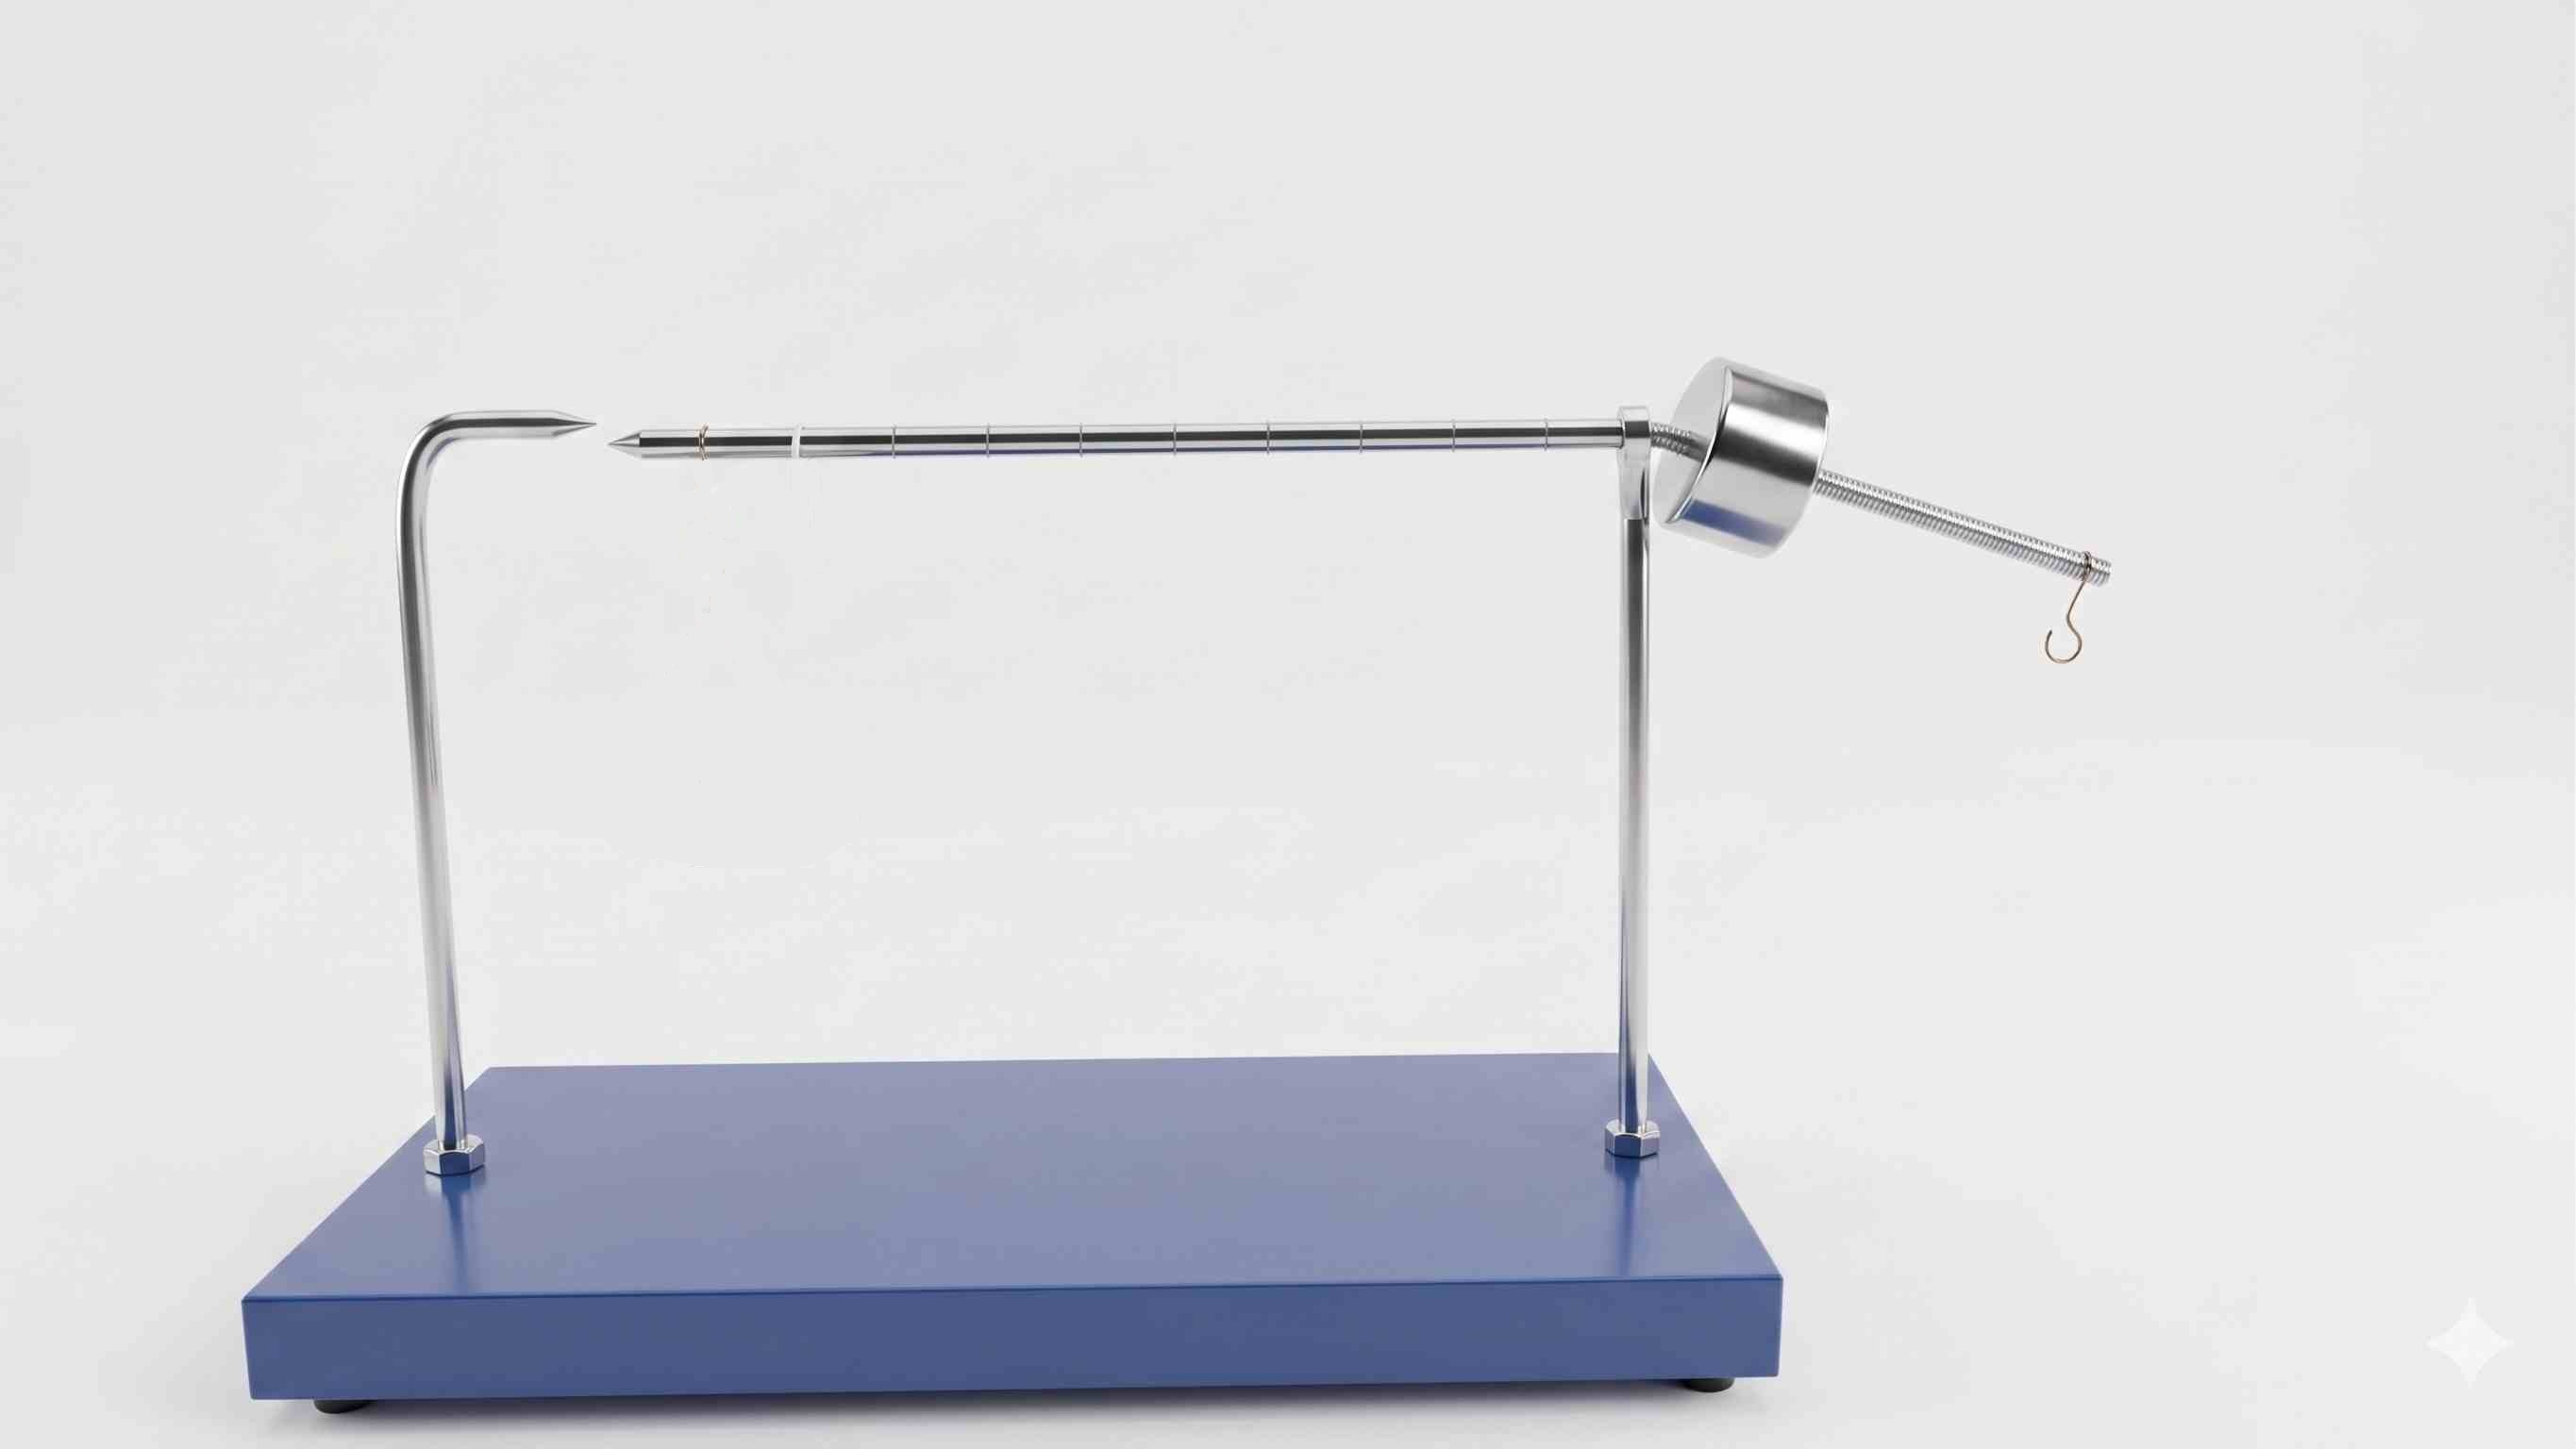
\includegraphics[width=0.50\linewidth]{Figures/balanza_mw.jpg}
    \caption{Balanza de Mohr--Westphal con jinetillos empleada en el
    primer método.}
    \label{fig:balanza_mw}
\end{figure}

%% --- Material 1 ---
\subsection{Anillo metálico}

\begin{itemize}
    \item \textbf{Descripción y función:} Anillo circular de aluminio
    suspendido del brazo mayor de la balanza. Al sumergirse en la superficie
    del agua forma una película que ejerce la fuerza de tensión superficial
    a lo largo de sus circunferencias interna y externa.
    \item \textbf{Precauciones:} Asegurarse de que el anillo quede paralelo
    a la superficie del líquido antes de iniciar la medición.
\end{itemize}

\begin{figure}[H]
    \centering
    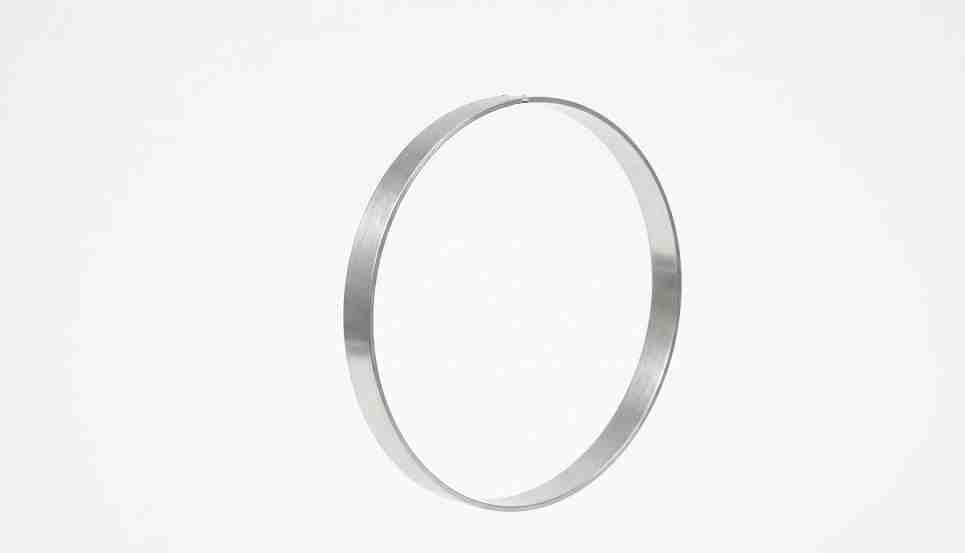
\includegraphics[width=0.50\linewidth]{Figures/anillo.jpg}
    \caption{Anillo metálico de aluminio empleado para formar la película
    de agua.}
    \label{fig:anillo}
\end{figure}

%% --- Material 2 ---
\subsection{Jinetillos}

\begin{itemize}
    \item \textbf{Descripción y función:} Pequeñas masas en forma de U que
    se colocan en las ranuras numeradas del brazo mayor para replicar el
    torque de la fuerza de tensión superficial una vez retirado el recipiente
    con agua.
    \item \textbf{Especificaciones:}
    \begin{itemize}
        \item Incertidumbre en masa: \qty{\pm 0{,}1}{g}
    \end{itemize}
    \item \textbf{Precauciones:} Registrar con exactitud la ranura en que se
    coloca cada jinetillo, pues el torque depende directamente de su
    posición.
\end{itemize}

\begin{figure}[H]
    \centering
    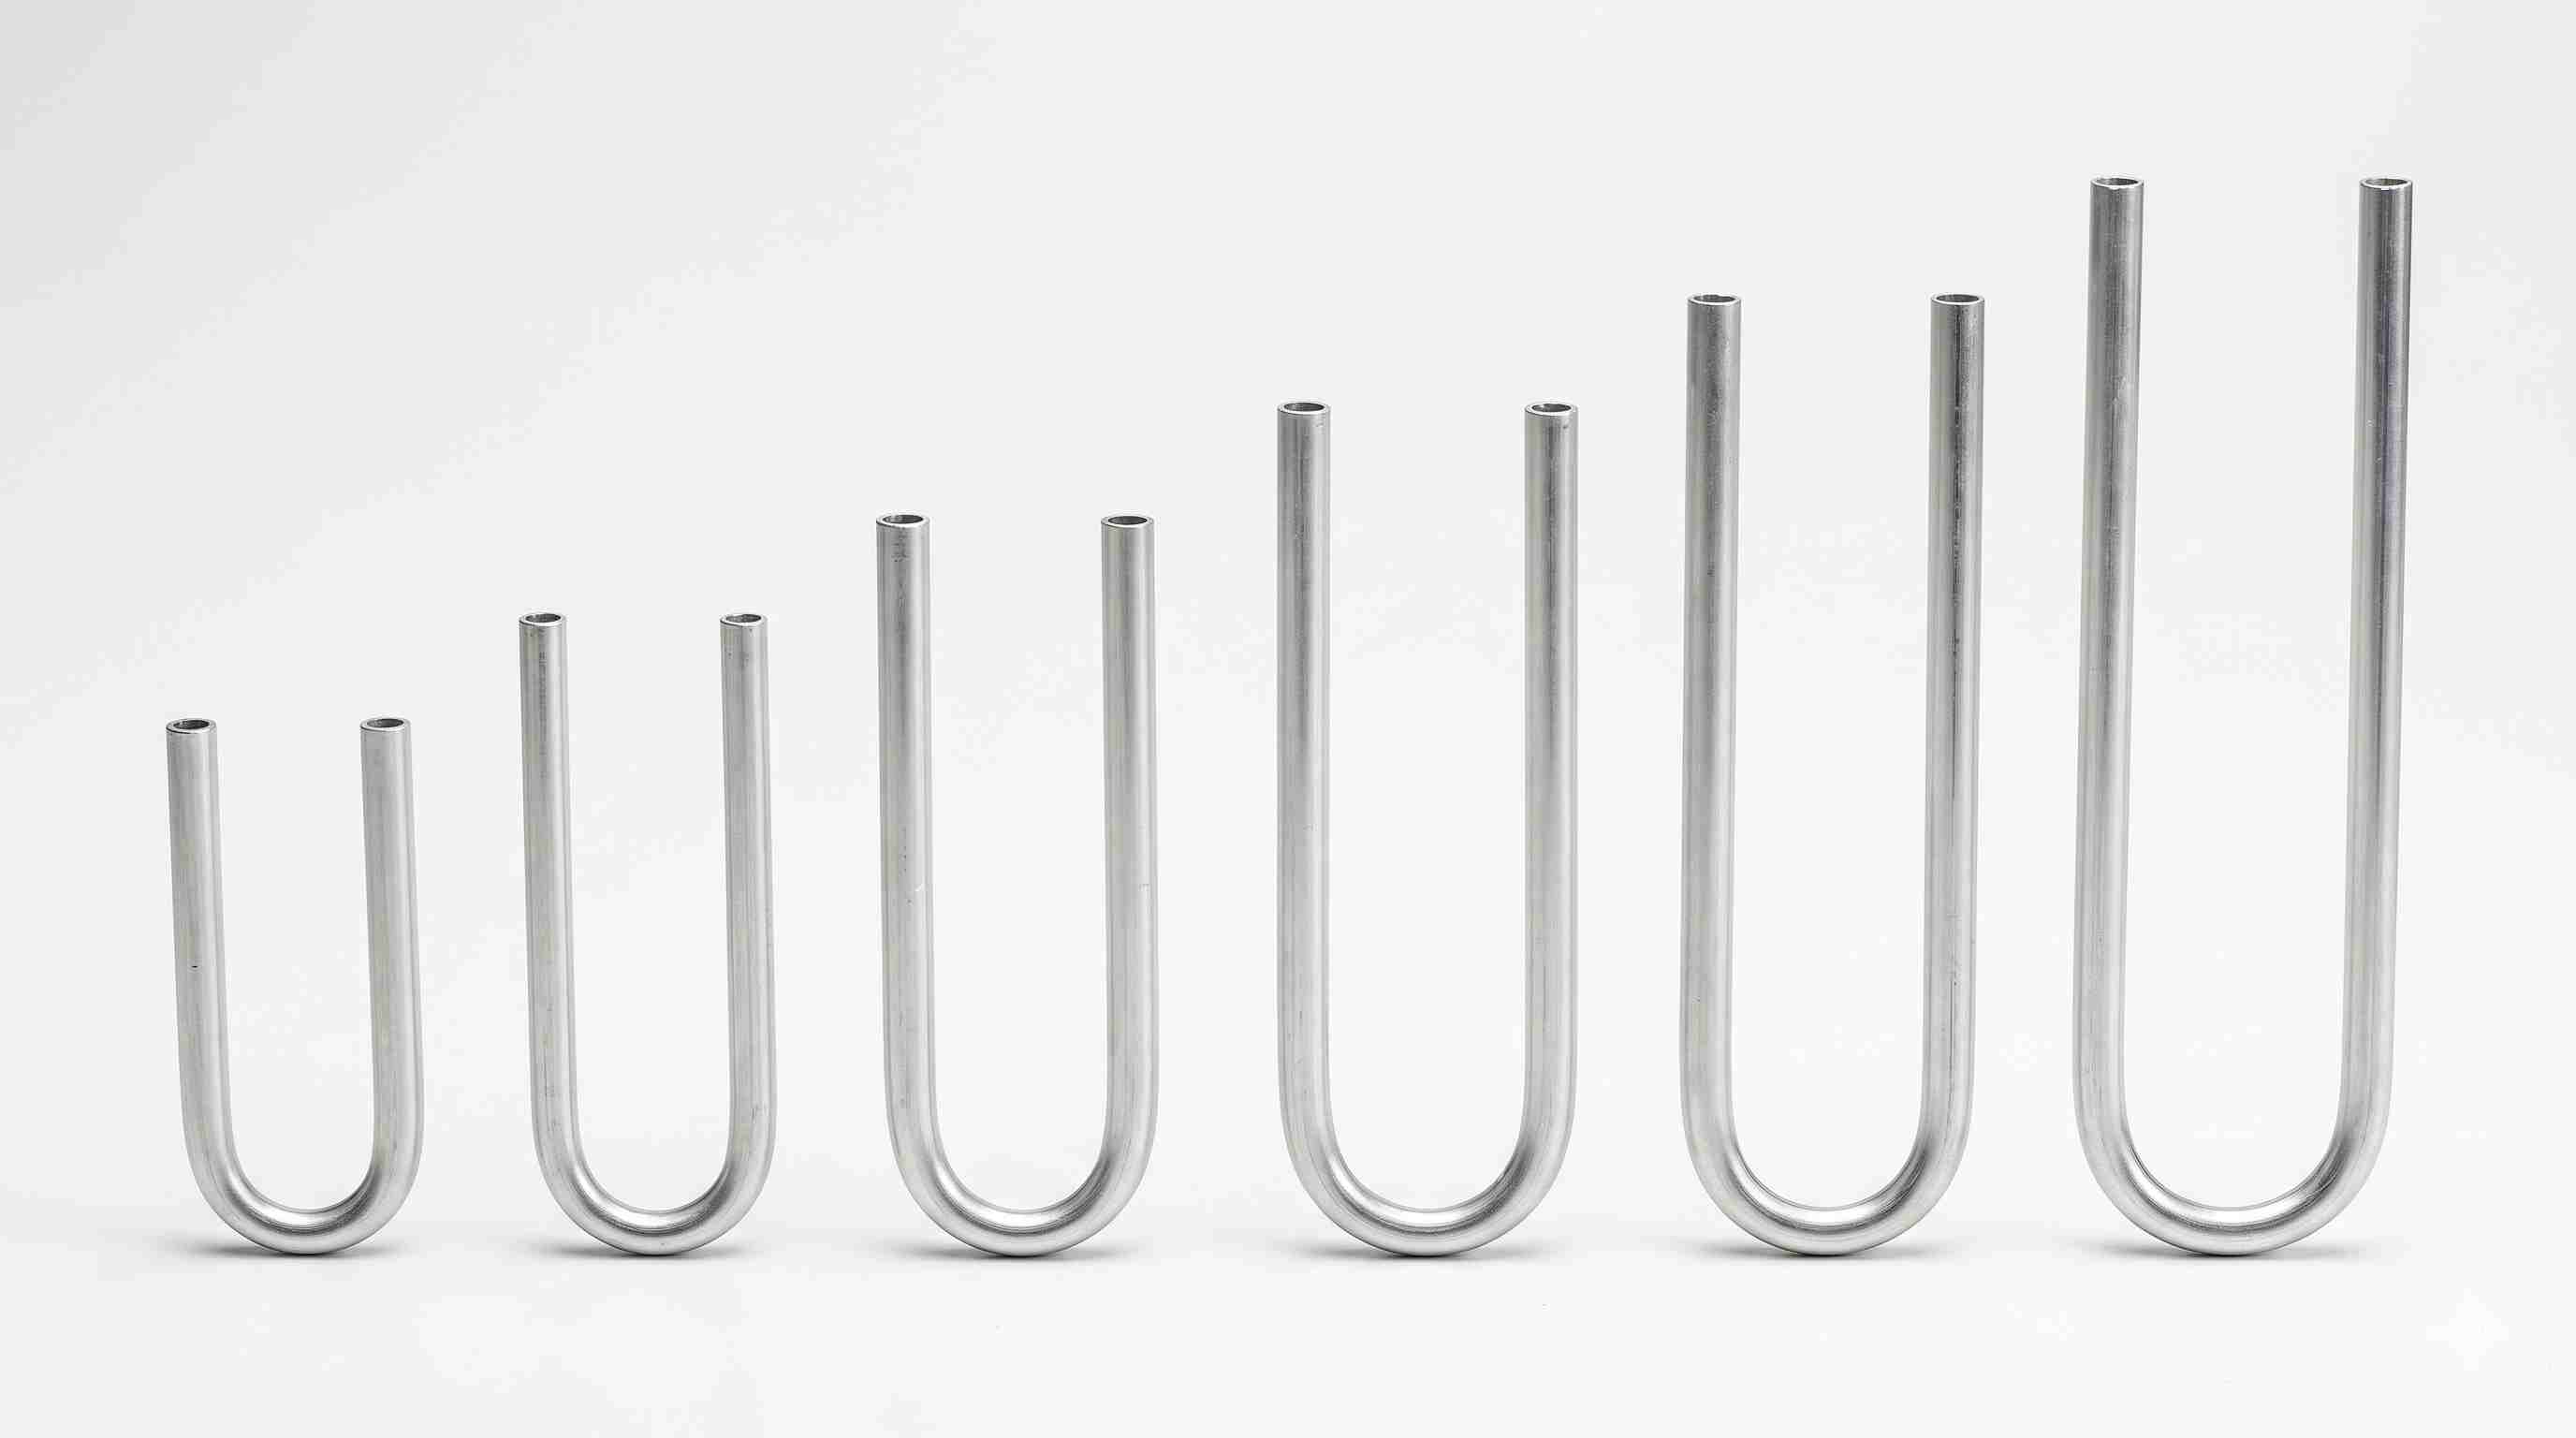
\includegraphics[width=0.50\linewidth]{Figures/jinetillos.jpg}
    \caption{Jinetillos de aluminio utilizados para equilibrar la balanza.}
    \label{fig:jinetillos}
\end{figure}

%% --- Instrumento 1 ---
\subsection{Vernier (calibrador)}

\begin{itemize}
    \item \textbf{Descripción y función:} Instrumento de medición utilizado
    para determinar los radios interno y externo del anillo, así como las
    dimensiones geométricas $a$, $b$ y $h$ de la película jabonosa en el
    segundo método.
    \item \textbf{Especificaciones:}
    \begin{itemize}
        \item Resolución: \qty{0{,}05}{mm}
        \item Incertidumbre: \qty{\pm 0{,}05}{mm}
    \end{itemize}
    \item \textbf{Precauciones:} Verificar el cero del vernier antes de cada
    medición. Medir siempre en la zona media del objeto.
\end{itemize}

\begin{figure}[H]
    \centering
    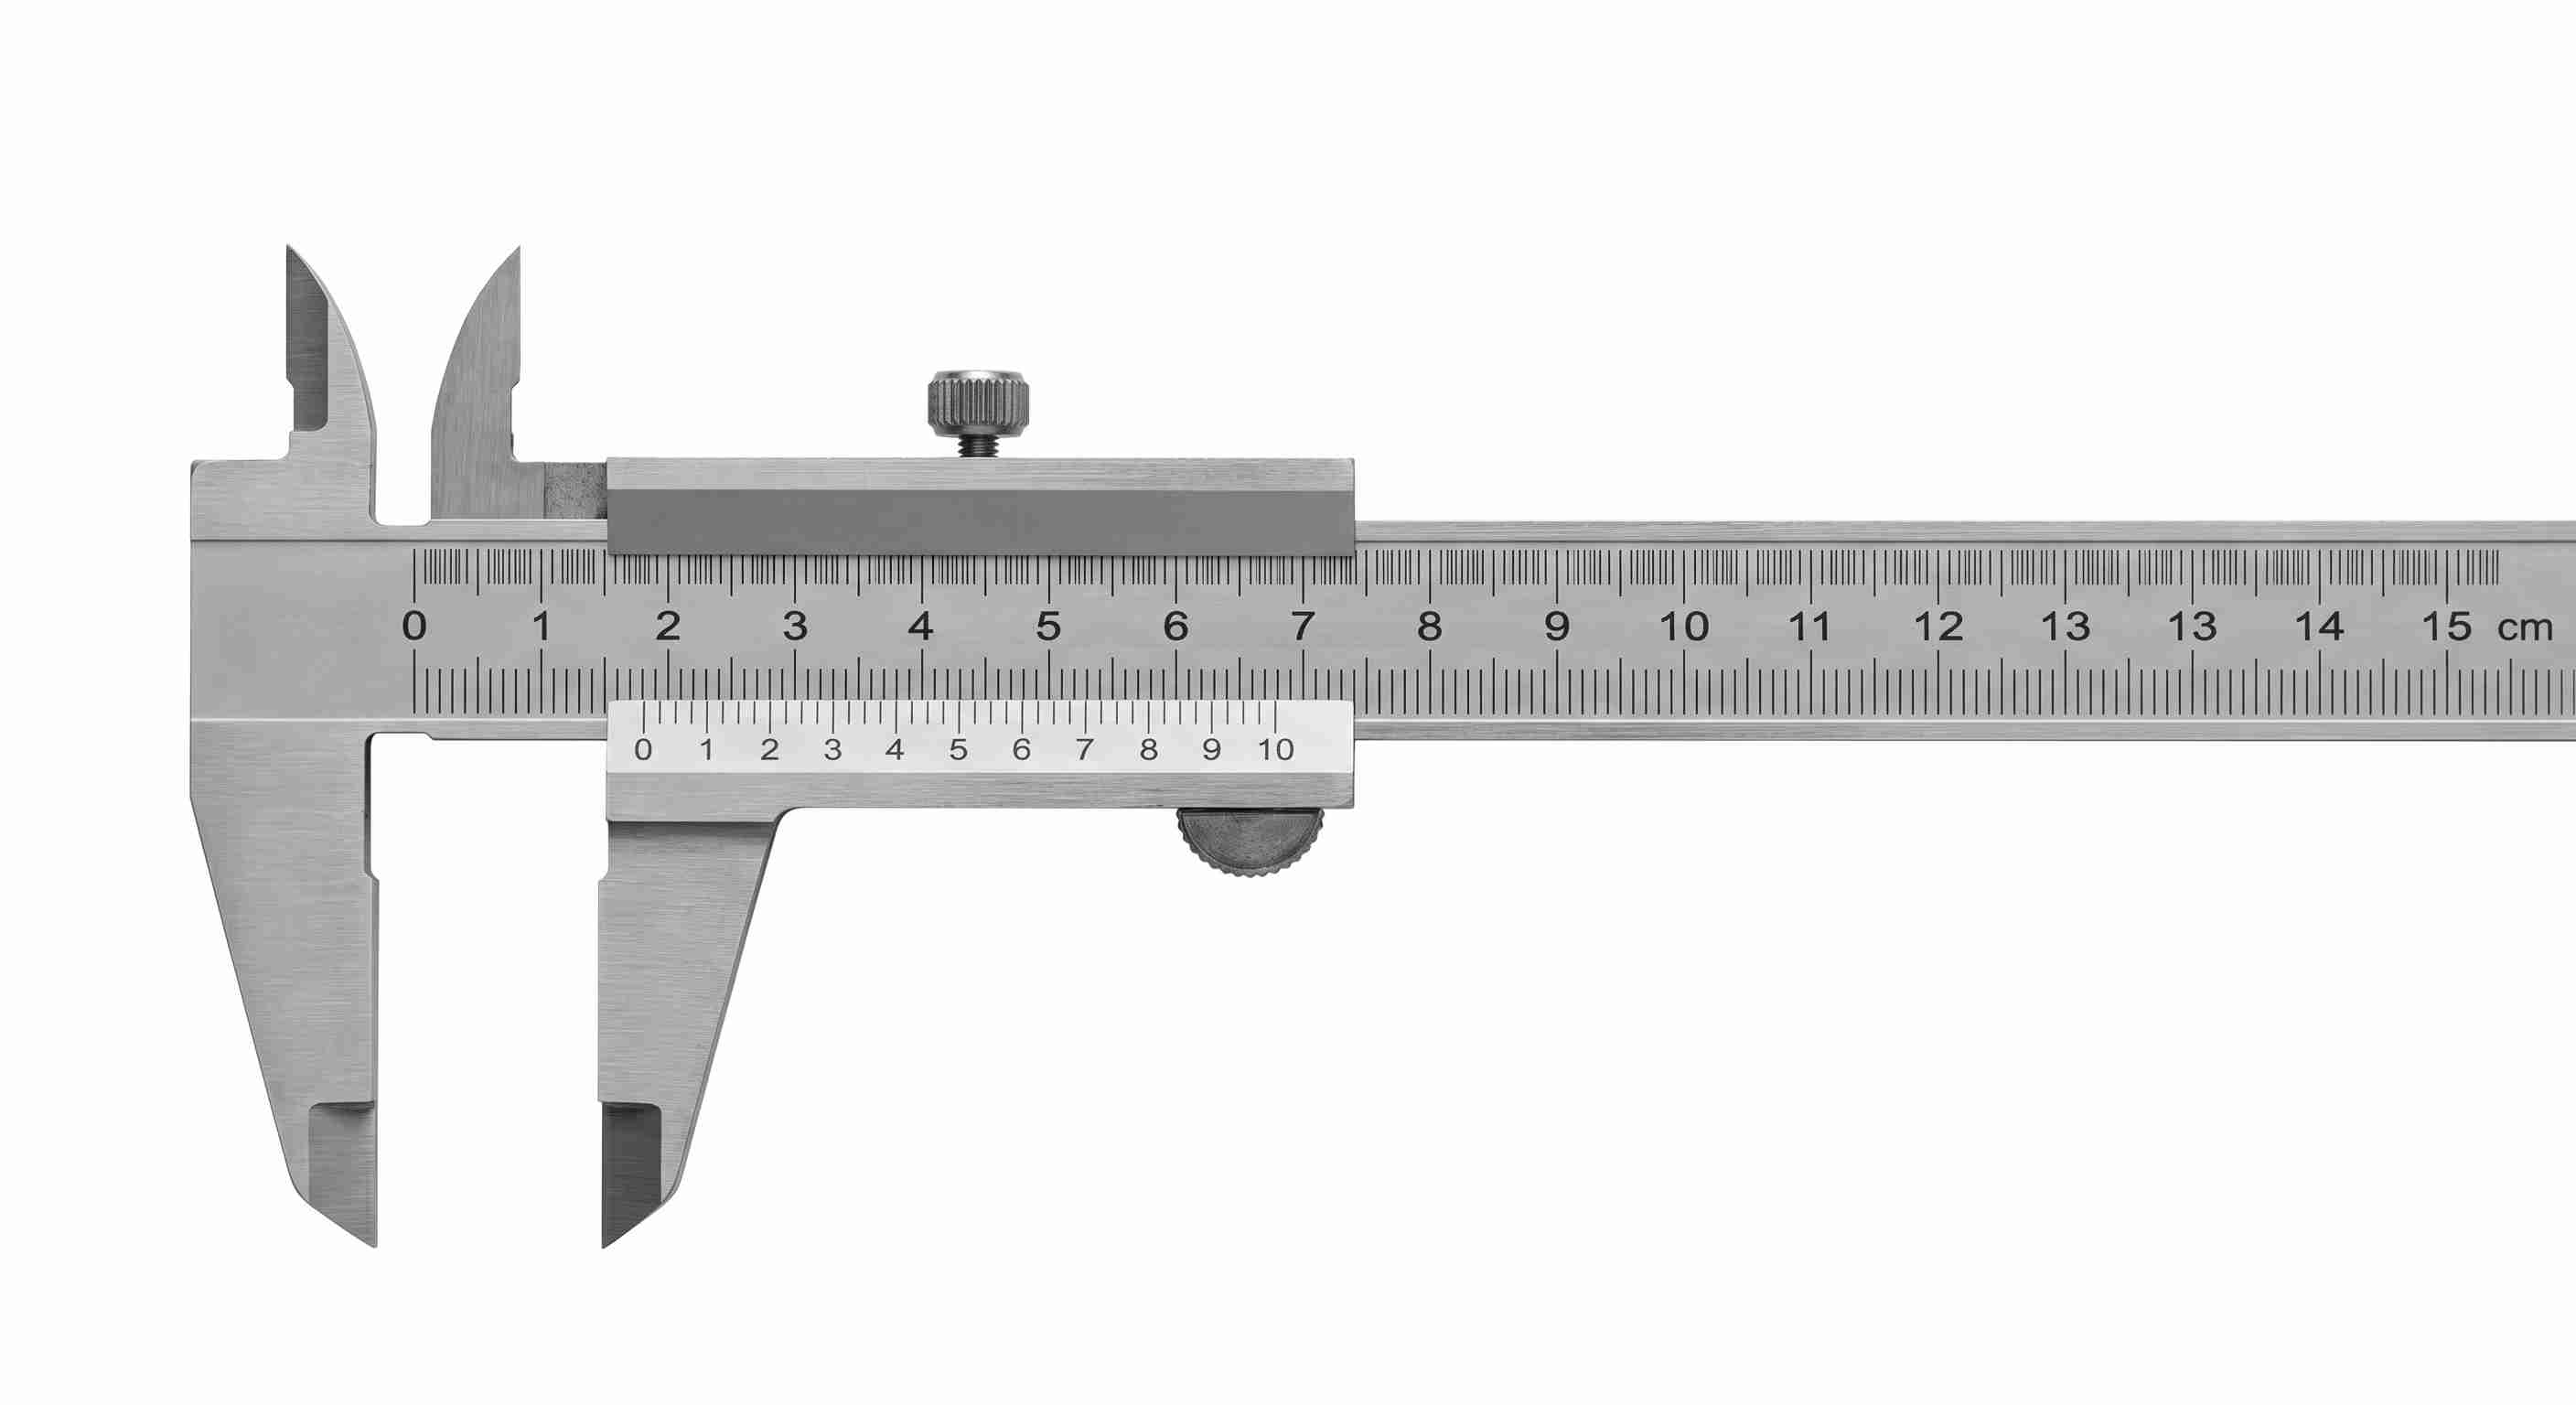
\includegraphics[width=0.50\linewidth]{Figures/vernier.jpg}
    \caption{Vernier (calibrador) empleado para la medición de dimensiones
    geométricas.}
    \label{fig:vernier}
\end{figure}

%% --- Material 3 ---
\subsection{Dispositivo de tubitos con hilo}

\begin{itemize}
    \item \textbf{Descripción y función:} Sistema formado por dos tubitos de
    vidrio unidos lateralmente por un hilo delgado y liviano. Uno de los
    tubos lleva un alambre transversal que permite suspender el conjunto.
    Al sumergirse en solución jabonosa y retirarse, se forma una película
    cuya contracción curva el hilo inferior, permitiendo calcular $\gamma$
    mediante la Ec.~\eqref{eq:gamma_m2}.
    \item \textbf{Precauciones:} Mantener el sistema horizontal al
    suspenderlo. Realizar las mediciones geométricas inmediatamente después
    de retirar el dispositivo de la solución, antes de que la película se
    evapore.
\end{itemize}

\begin{figure}[H]
    \centering
    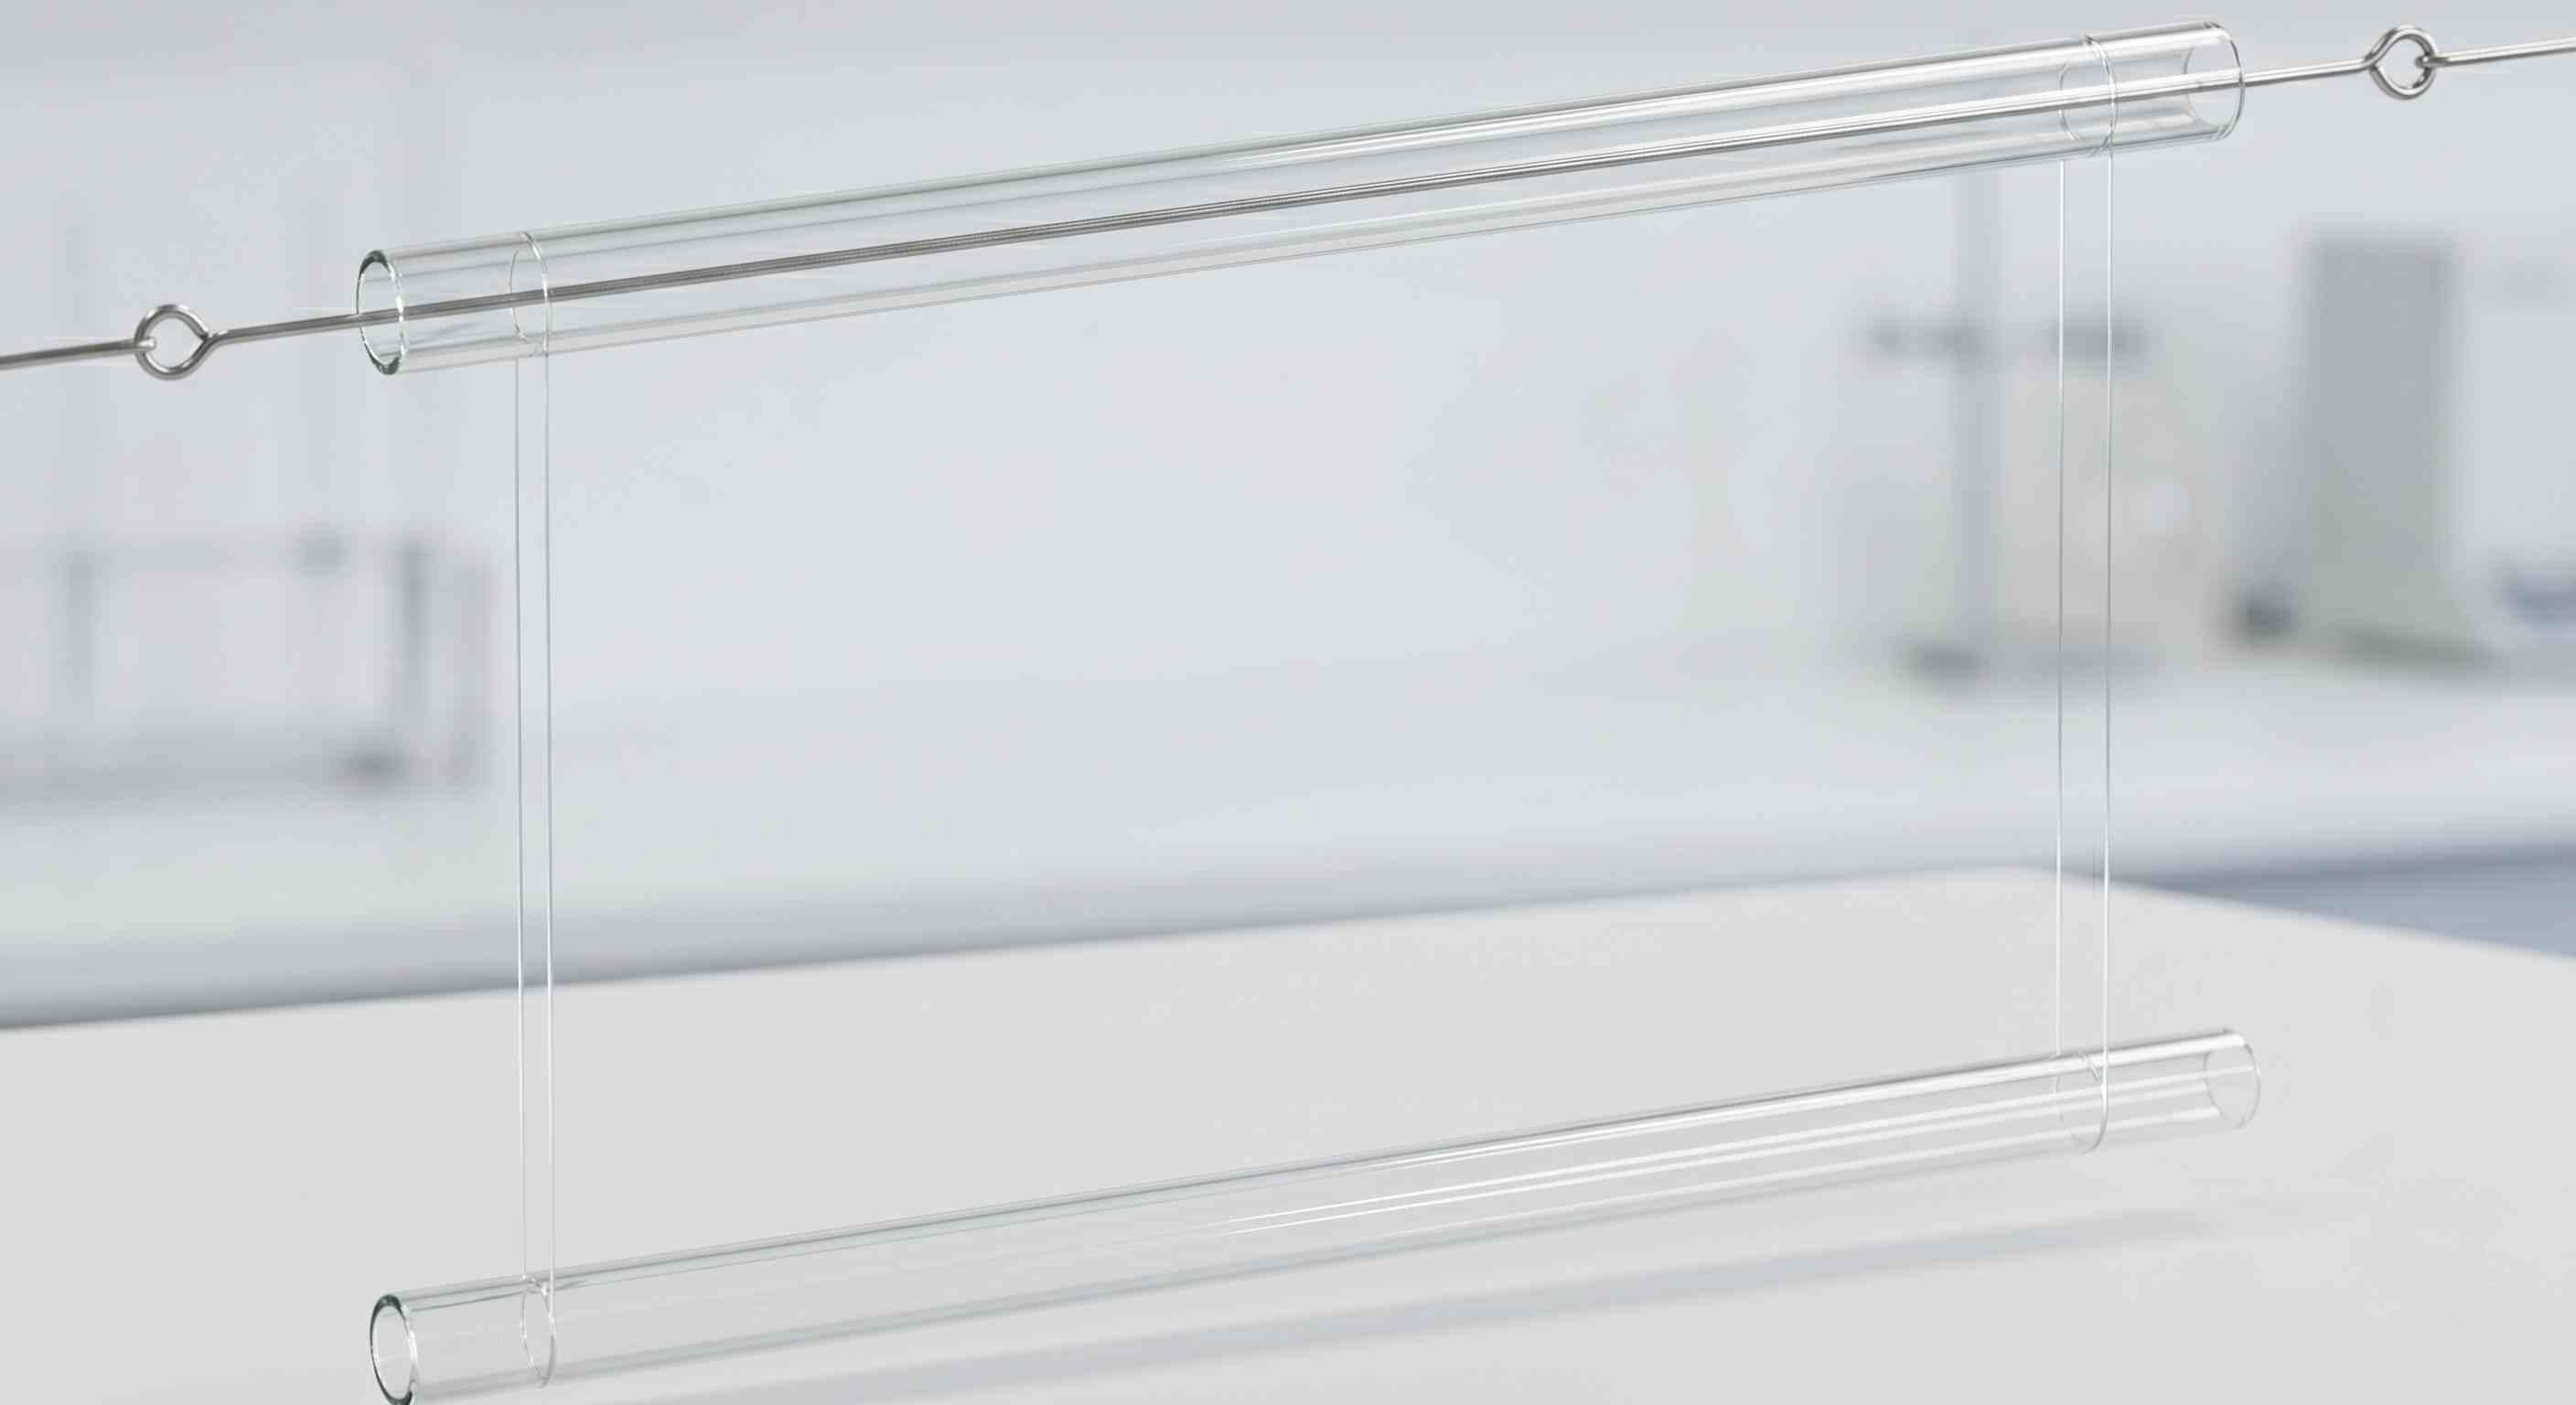
\includegraphics[width=0.50\linewidth]{Figures/tubitos.jpg}
    \caption{Dispositivo de tubitos con hilo empleado en el segundo método.}
    \label{fig:tubitos}
\end{figure}

%% --- Material 4 ---
\subsection{Recipientes, soluciones y accesorios}

\begin{itemize}
    \item \textbf{Descripción y función:} Recipiente con agua corriente para
    el primer método y recipiente con solución jabonosa (agua con detergente)
    para el segundo. Un vasito de plástico actuó como balde receptor de arena
    en el brazo menor de la balanza, y una pipeta permitió añadirla de forma
    controlada y gradual.
    \item \textbf{Precauciones:} No contaminar el recipiente de agua pura con
    detergente. Agregar la arena muy lentamente para evitar sobrepasar el
    punto de desprendimiento del anillo.
\end{itemize}

\begin{figure}[H]
    \centering
    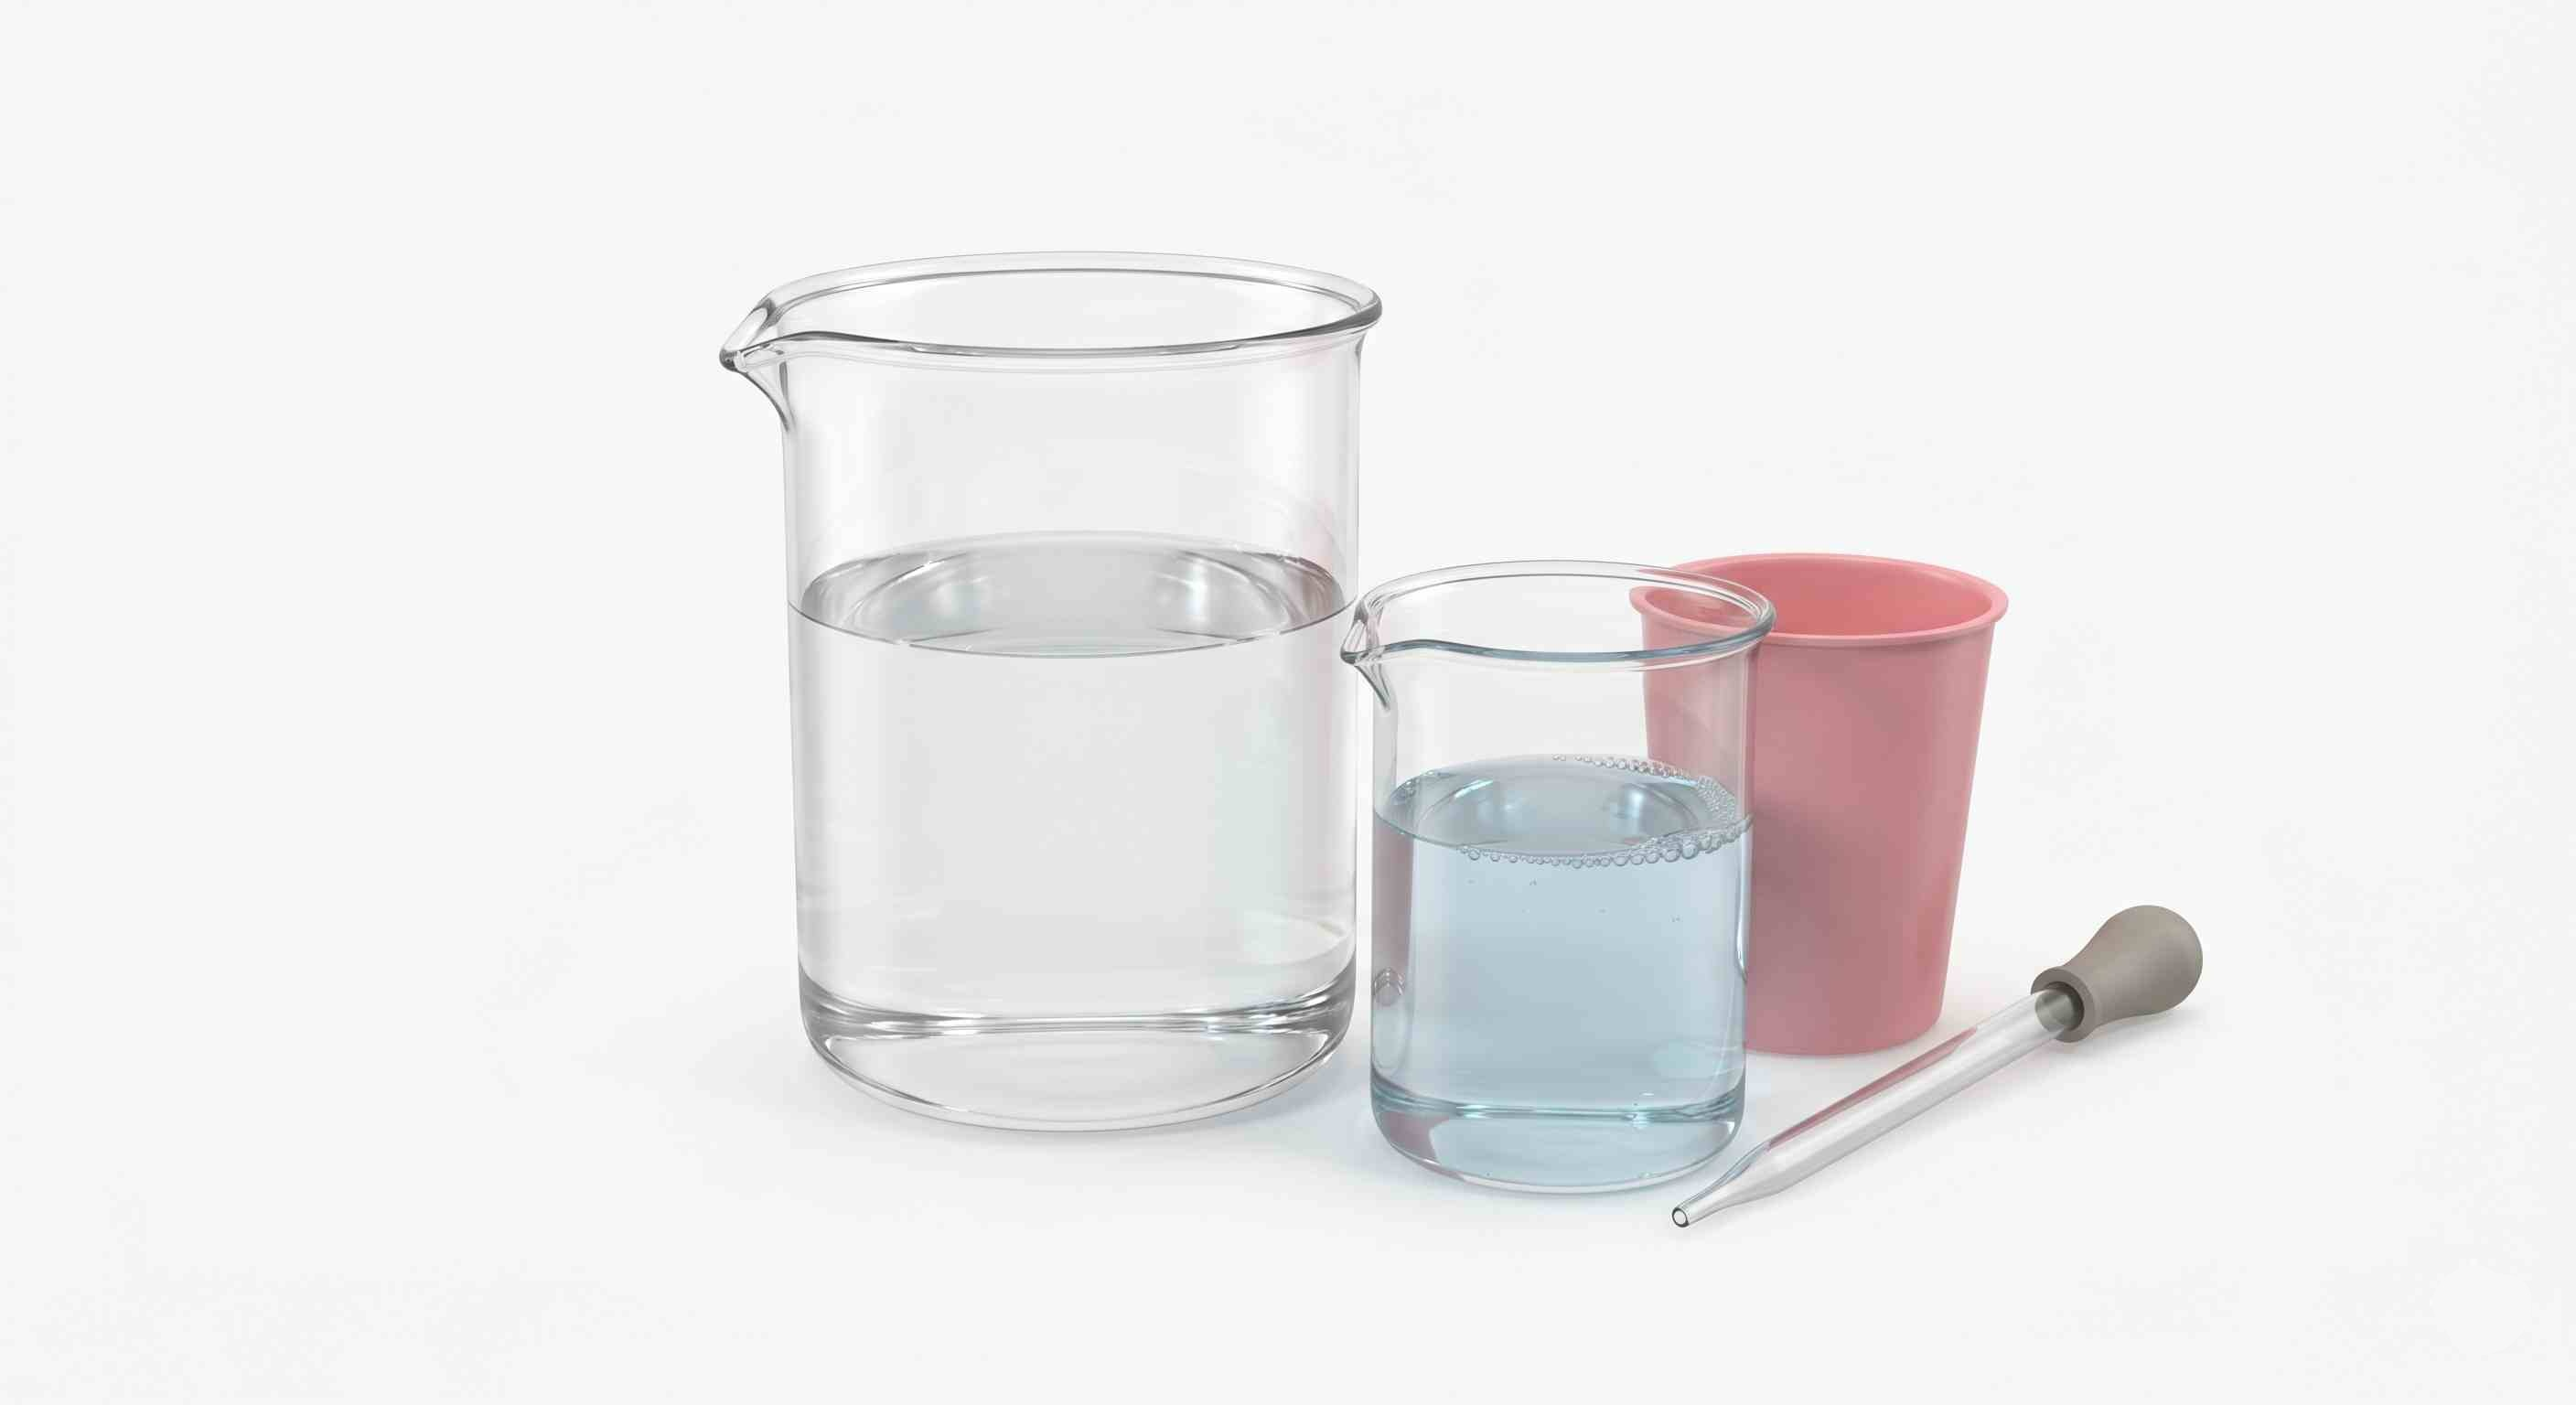
\includegraphics[width=0.50\linewidth]{Figures/recipientes.jpg}
    \caption{Recipientes y accesorios empleados en el experimento.}
    \label{fig:recipientes}
\end{figure}

%% --- Instrumento 2 ---
\subsection{Balanza de precisión}

\begin{itemize}
    \item \textbf{Descripción y función:} Instrumento compartido por toda la
    clase, utilizado para determinar la masa de los jinetillos y del tubo
    inferior del dispositivo de hilo.
    \item \textbf{Especificaciones:}
    \begin{itemize}
        \item Incertidumbre: \qty{\pm 0{,}1}{g}
    \end{itemize}
    \item \textbf{Precauciones:} Nivelar la balanza antes de cada uso y
    coordinar el turno de medición con los demás grupos.
\end{itemize}

\begin{figure}[H]
    \centering
    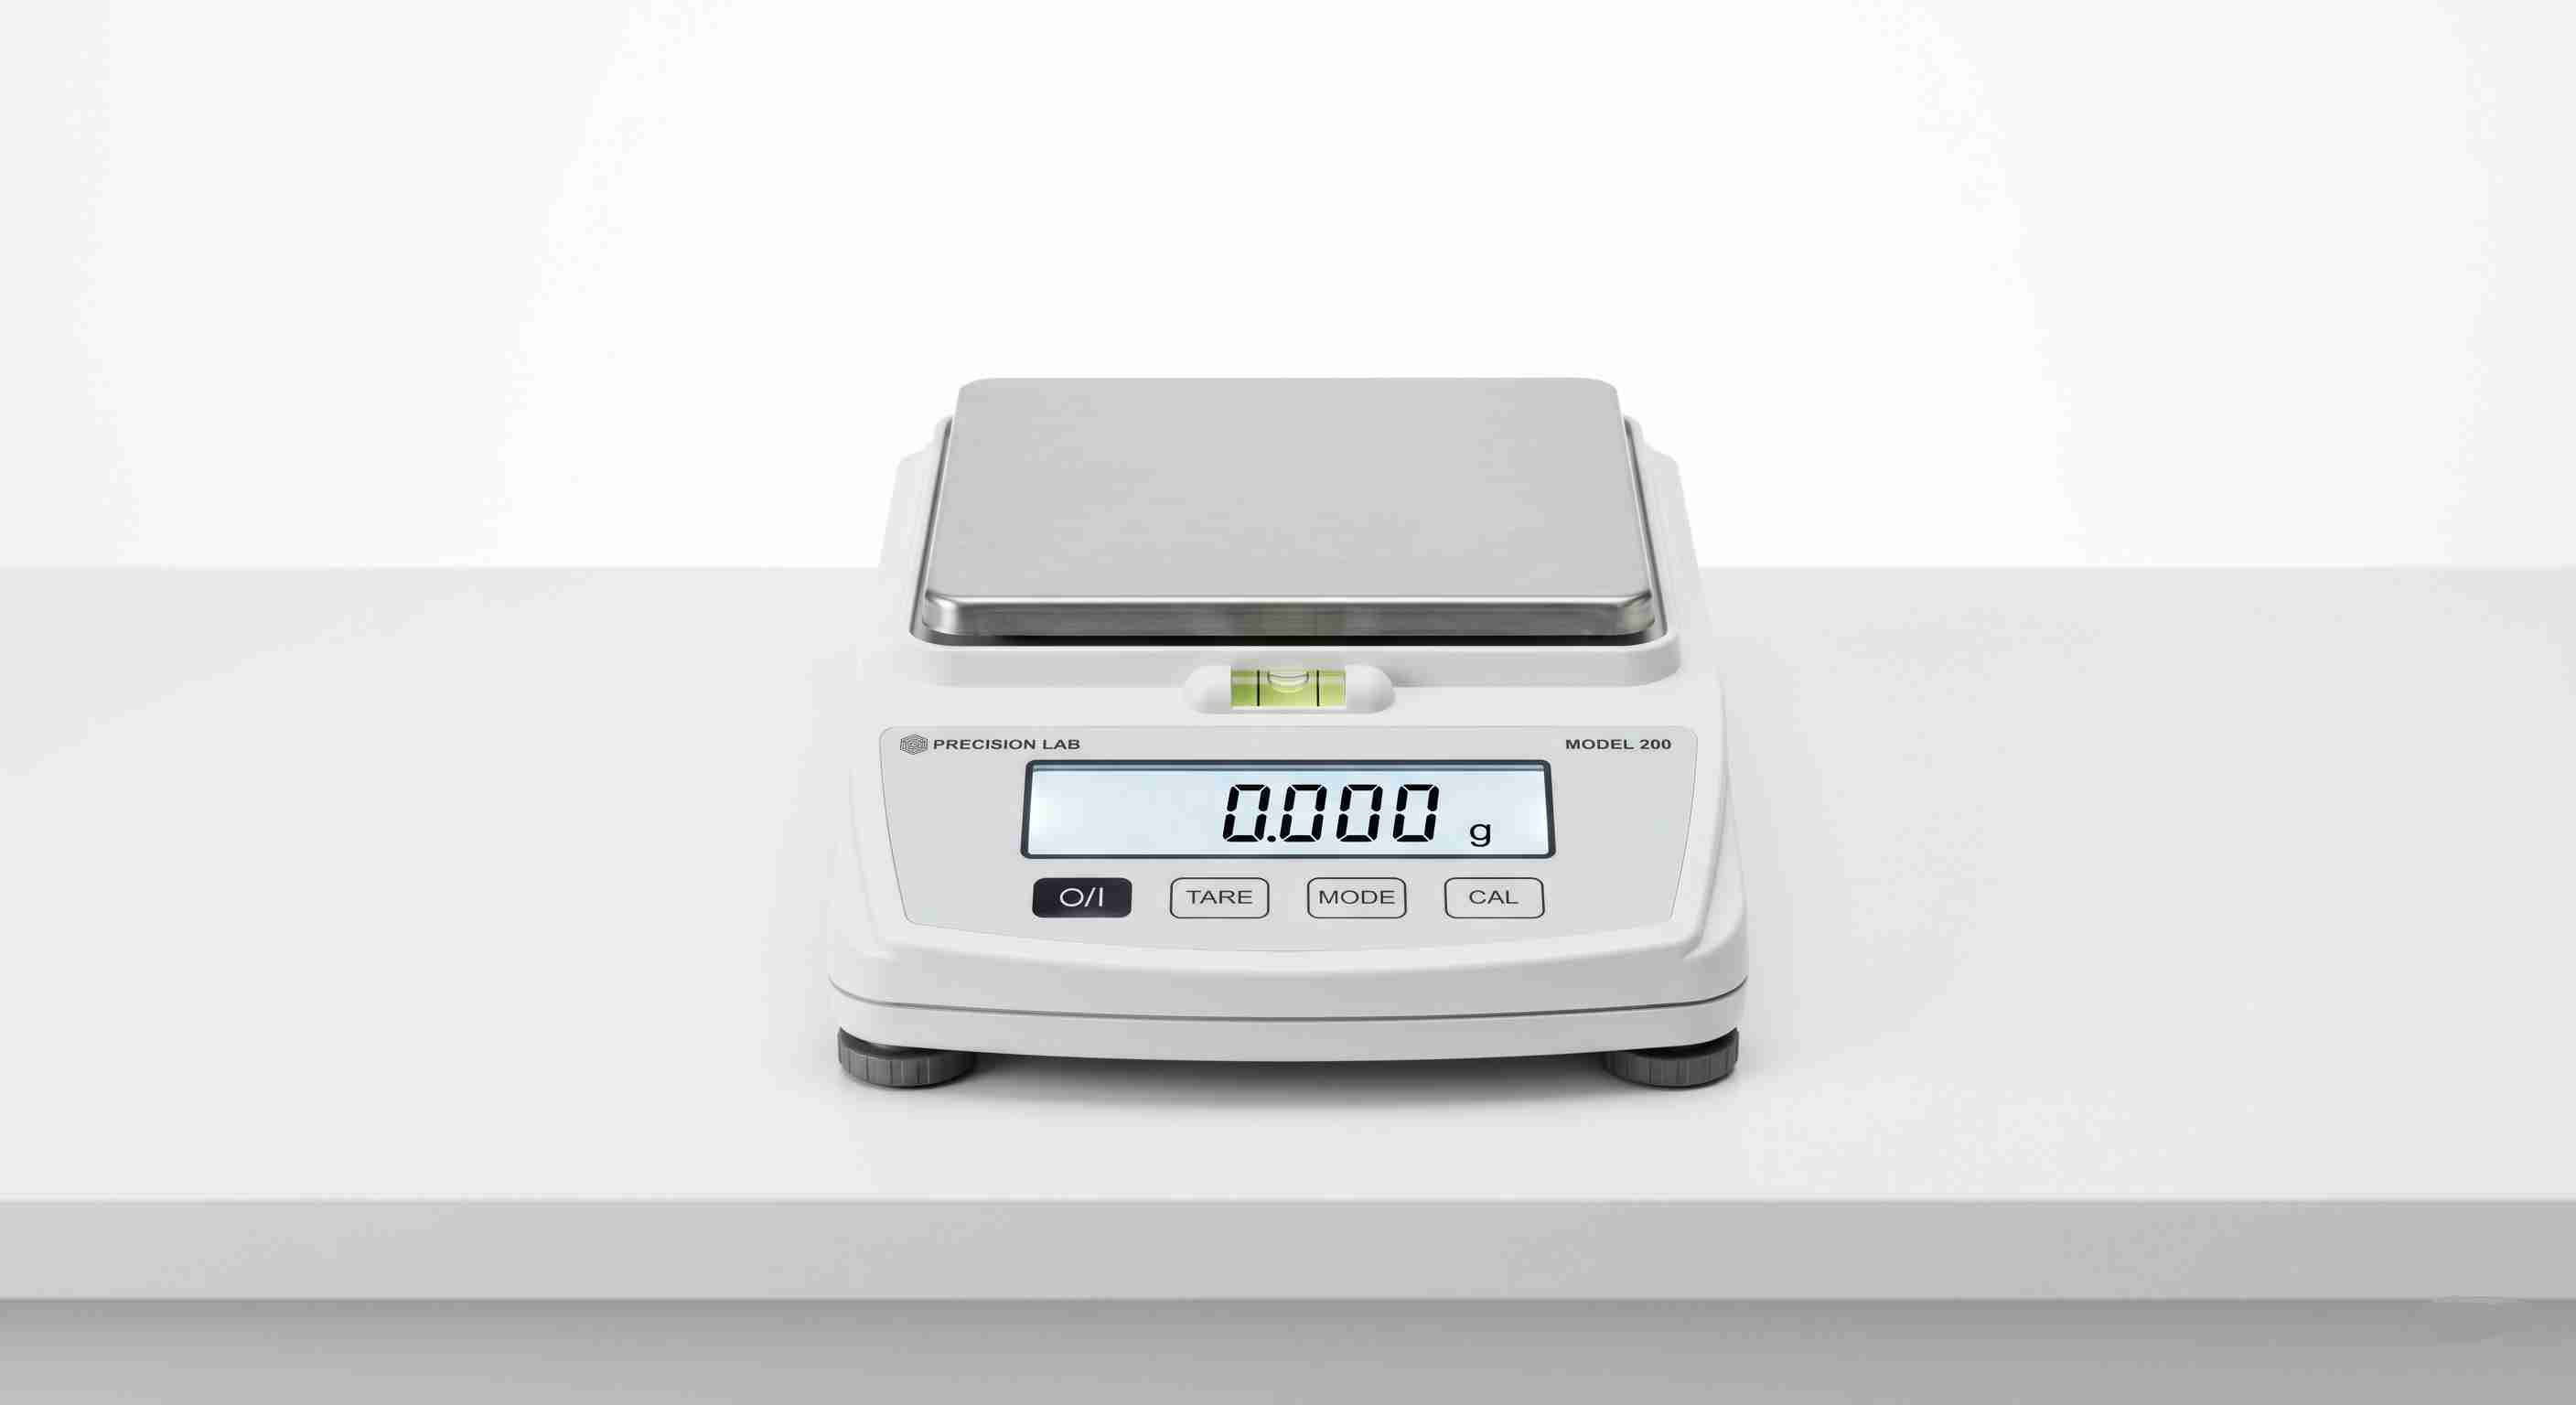
\includegraphics[width=0.50\linewidth]{Figures/balanza_prec.jpg}
    \caption{Balanza de precisión empleada para la medición de masas.}
    \label{fig:balanza_prec} 
\end{figure}
